\begin{frame}[allowframebreaks]{Outline}
\frametitle{Bitonic Banyan Network}
 \begin{itemize}
  \item Self routing property of a Bitonic-Banyan network \\
  \item Configuration contians a Bitonic network cascased with a Banyan Tree. \\
  \item Bitonic network configuration remains the same except the switches are modified. \\
  \item Below are the different scenarios for the modified switches\\
   \begin{figure}[!ht]
    %\includegraphics[width=8.35cm, height=7cm]{figures/RouterNetwork}
    \includegraphics[width=7cm, height=2cm]{figures/Batcher_Switches}
    \caption{Modified switches for Bitonic network }
  \end{figure}
  \item The \textit{Normal switch} and \textit{Modified switch} are mutliplexed w.r.t the \textit{VALID} bit.
  \item The below figure shows the implemention of switching element.
  \begin{figure}[!ht]
    %\includegraphics[width=8.35cm, height=7cm]{figures/RouterNetwork}
    \includegraphics[width=7cm, height=3.5cm]{figures/Switching_Element}
    \caption{Swithing element of Bitonic Network}
  \end{figure}
  \item A N input Banyan network characterized of $O( N.log_{2}(N)$ switching elements and $O(log_{2}(N)$ stages \\
  \item A Banyan switch routes the input based on the $i^{th}$ bit of the header. In our case the \textit{Target-Address} \\
  and  $i$ is the index of the Banyan stage.
  \item In our case to handle the invalid addresses, the bit controlled algorithm is modified as shown in the following figure \\
   \begin{figure}[!ht]
    %\includegraphics[width=8.35cm, height=7cm]{figures/RouterNetwork}
    \includegraphics[width=9cm, height=0.8cm]{figures/Banyan_Switches}
    \caption{ Different senarios of a banyan switch}
  \end{figure}
  \item  A Banyan newtwork is always collision free if the input sequences are sorted ascending.\\
  \item  The initial Bitnoic stage ensures ascending sequence at the input of the Banyan thus gurantee a collision free Banyan network. \\
  \item  The below figures depicts a screen capture of the VHDL Simulation\\
   \begin{figure}[!htb]
  \minipage{0.32\textwidth}
  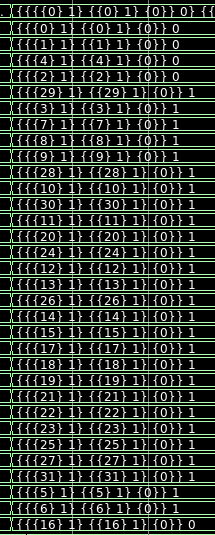
\includegraphics[width=2.2 cm, height=5.5cm]{figures/1}
  \caption{Input sequence}
  \endminipage\hfill
  \minipage{0.32\textwidth}
  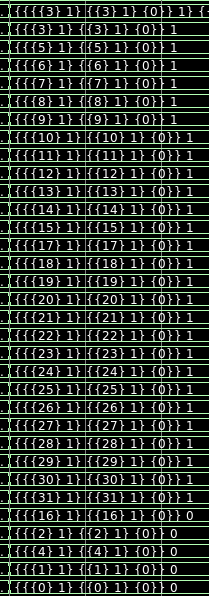
\includegraphics[width=2.2 cm, height=5.5 cm]{figures/2}
  \caption{After Bitonic stage}
  \endminipage\hfill
  \minipage{0.32\textwidth}%
  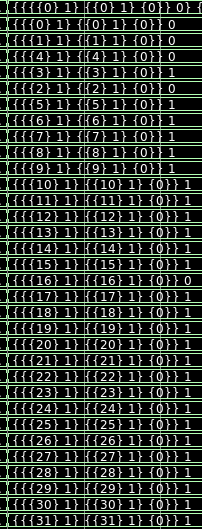
\includegraphics[width=2.2cm, height=5.5cm]{figures/3}
  \caption{After Banyan tree}
  \endminipage
  \end{figure}
  \item From benchmarks its has been already proven tha for $N > 8$ the latency due to combinatorial depth of a Bitonic network is more that when it is piplelined.\\
  \item Implemented 5 stage pipleline for th Bitonic network also a 5 stage pipeline for the Banyan network.\\
  \item The complete design of the DTN is shown as below. \\
    \begin{figure}[!ht]
    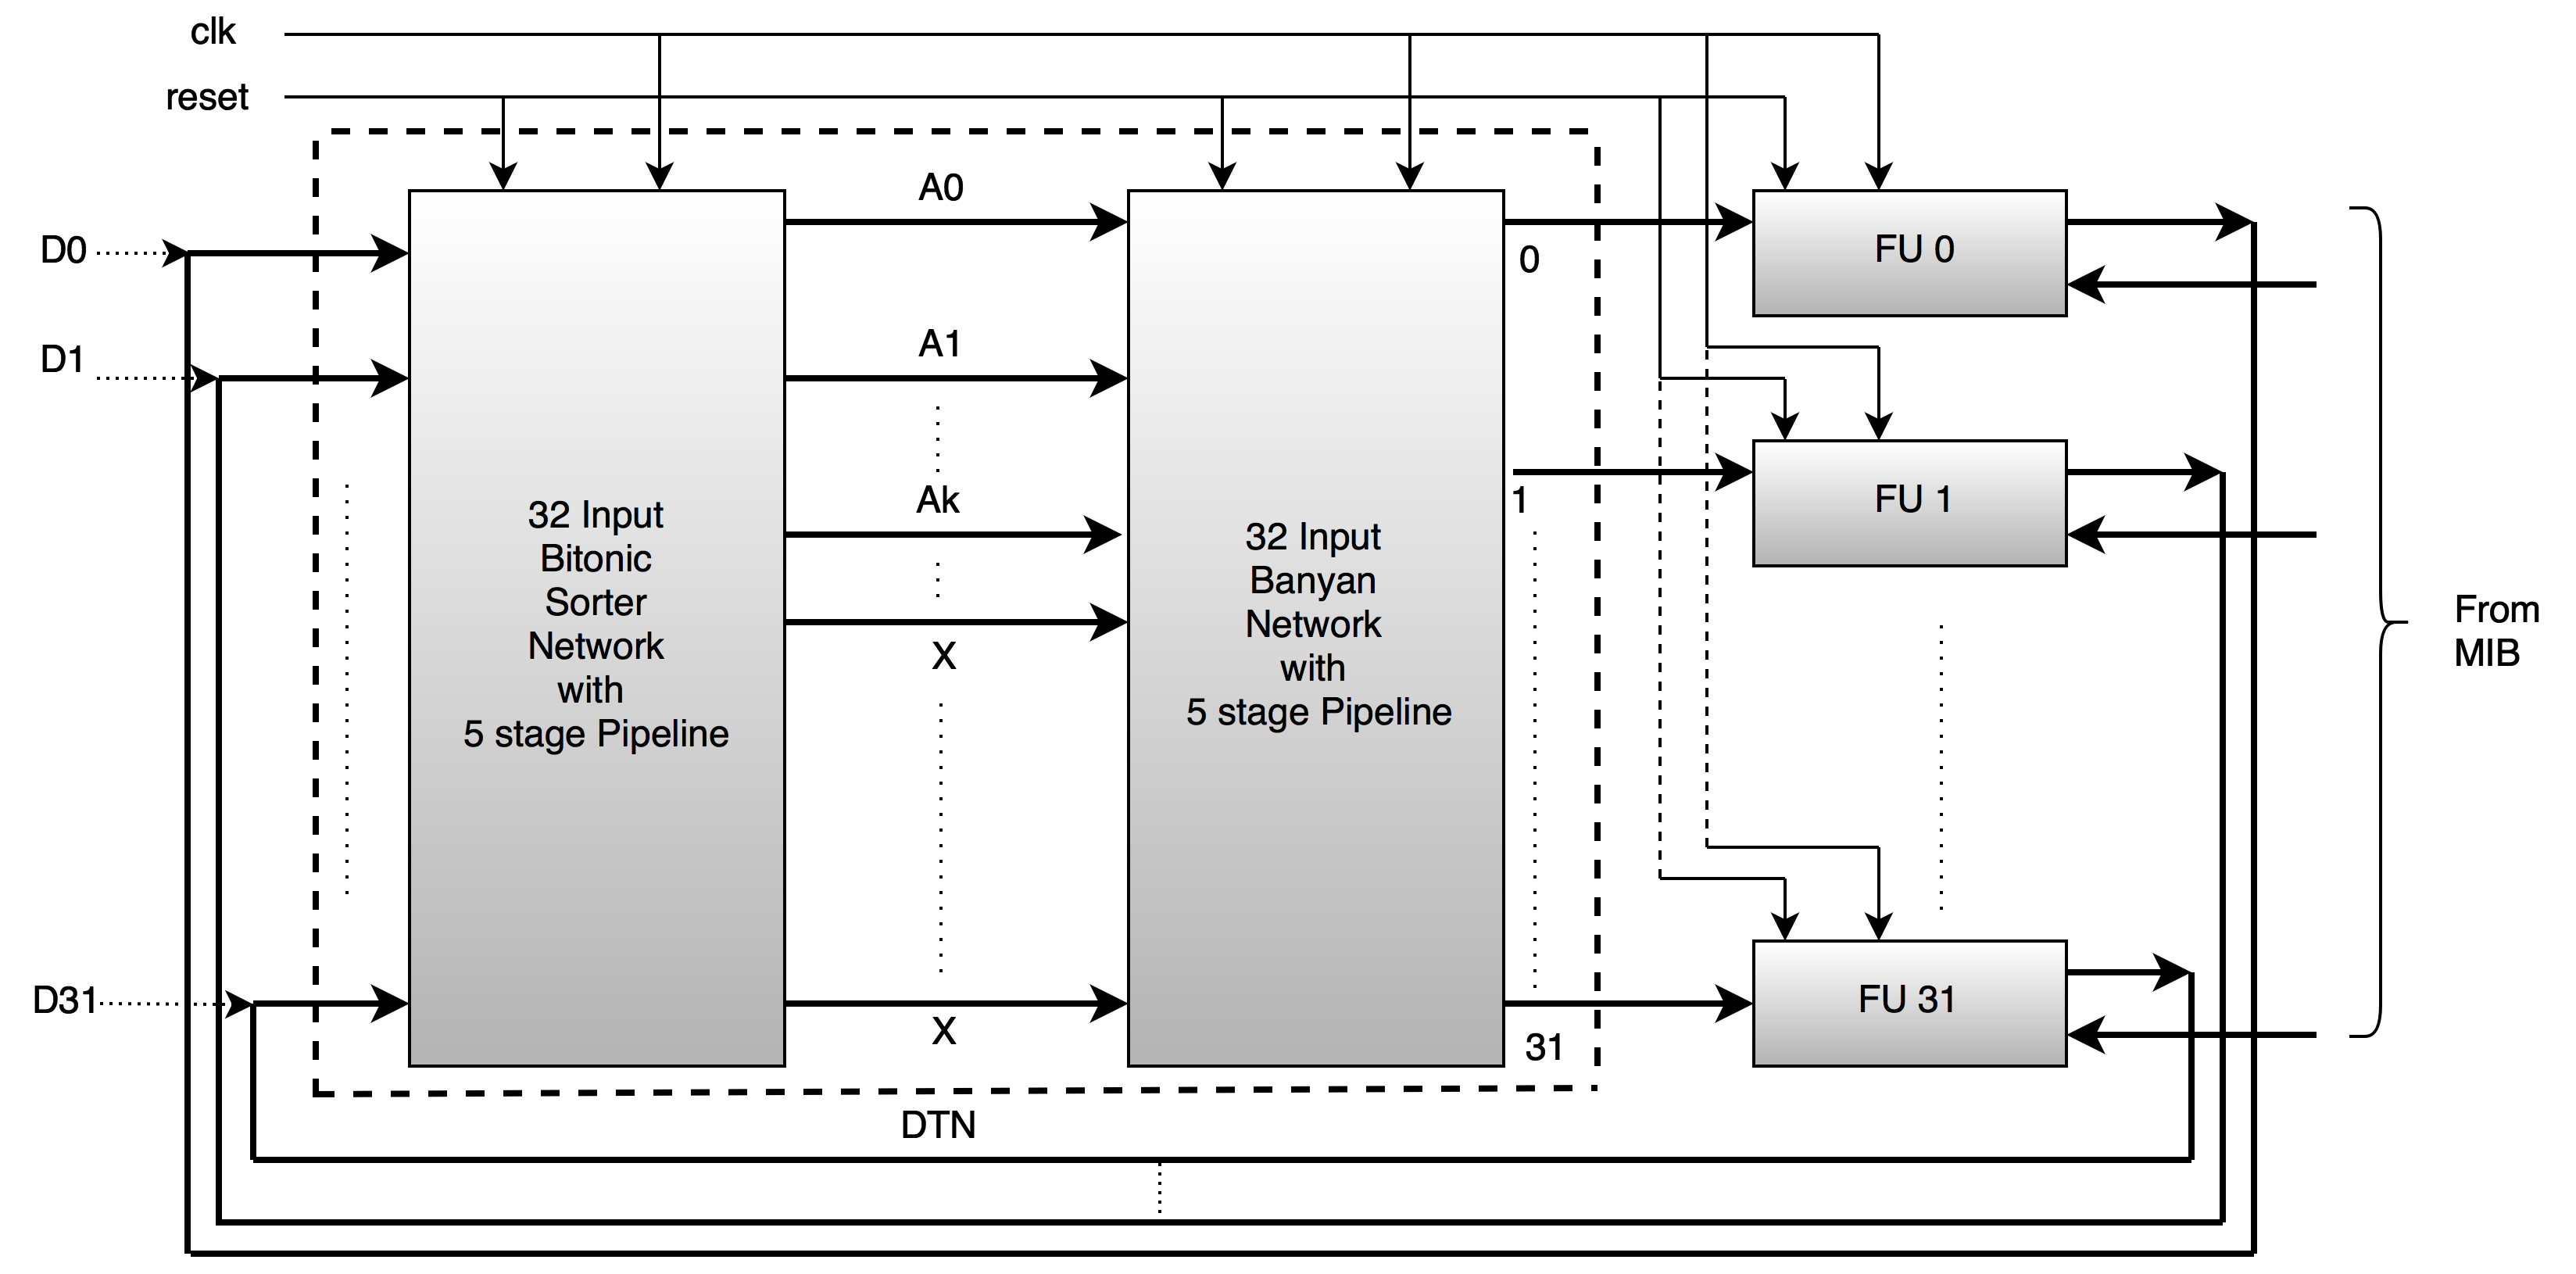
\includegraphics[width=9cm, height=5cm]{figures/Batcher_Banyan_Combined}
    \caption{Bitnoic-Banyan DTN of SCAD architecture}
  \end{figure}
  \end{itemize}
\end{frame}
